\documentclass[12pt,a4paper,oneside]{article}
\usepackage{amsmath,amsthm}
\usepackage{graphicx}
\usepackage{ctex}
\usepackage{float}
\usepackage{subfigure,subcaption}
\usepackage{caption}

\title{计算方法编程作业2实验报告}
\author{张博厚 PB22071354}
\date{}

\begin{document}
\maketitle
\tableofcontents
\newpage
\section{实验目的}
通过C++语言实现两种求解线性方程组的算法: 列主元Gauss消元法与Gauss-Seidel迭代,
分别将所求结果与真实值比较, 分析两种算法的表现.
\section{实验内容}
对系数矩阵:
$$
A = 
\begin{pmatrix}
    -(2\epsilon+h) & \epsilon+h & & & \\
    \epsilon & -(2\epsilon+h) & \epsilon+h & & \\
    & \epsilon & -(2\epsilon+h) & \ddots & \\
    &        &   \ddots & \ddots & \epsilon+h \\
    &   &   & \epsilon & -(2\epsilon+h)
\end{pmatrix}
$$
对$\epsilon=1/0.1/0.01, a=0.5, n=100$, 分别使用两种算法求解, 并比较与精确值的误差.
\section{算法实现}
使用C++中的std::vector构造二维数组来表示矩阵, 以提供更好的可变大小扩展性和成员函数.对
涉及的数学运算(如计算矩阵范数,计算真实值)等, 调用了cmath标准库中的方法来进行.
\subsection{列主元消元,Gauss-Seidel迭代}
按照书中描述的算法步骤执行即可.
\subsection{计算精确值}
精确解已在实验文档中给出,由
\begin{equation}
    y = \dfrac{1-a}{1-e^{-1/\epsilon}}(1-e^{-\frac{x}{\epsilon}})+ax
\end{equation}
对每个离散的$x_i$, 分别代入上式计算精确值$y_i$,结果存入容器Tvalue中并返回.

\subsection{计算范数}
此函数用于计算两向量之差的无穷范数, 用于判断Guass-Seidel迭代的停止条件, 以及计算
最终结果与真实值的误差.
函数首先判断两输入向量a与b是否同维, 之后对两向量同时遍历, 找到$\mathbf{a}-\mathbf{b}
$中的绝对值最大分量.

\section{实验结果与分析}
分别令$\epsilon = 1,0.1, 0.01, 0.0001$, 所得结果如下:
\begin{figure}[H]
    \centering
    \subfigure[$\epsilon = 1$]{
        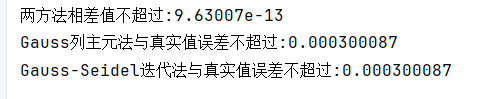
\includegraphics[scale = 0.65]{figs/1.png}
    }
    \subfigure[$\epsilon = 0.1$]{
        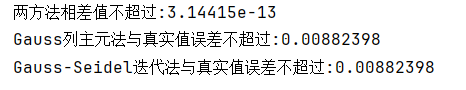
\includegraphics[scale = 0.6]{figs/0.1.png}
    }
    \hspace{0.5in} 
    \subfigure[$\epsilon = 0.01$]{
        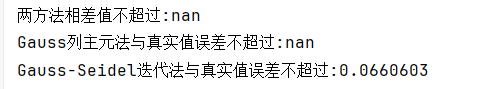
\includegraphics[scale = 0.65]{figs/0.01.png}
    }
    \subfigure[$\epsilon = 0.0001$]{
        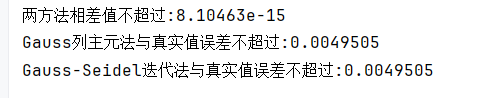
\includegraphics[scale = 0.6]{figs/0.0001.png}
    }
\end{figure}
其中, "误差不超过"是指将两向量做比较, 其差的无穷范数的最大值, 即将各自分量对比所得
的偏差最大值. 从结果可以看出, Gauss列主元消元法和Gauss-Seidel迭代法所得
结果一般相差不大, 与真实值相差$10^{-4}\sim 10^{-3}$数量级. 误差的主要来源
是差分法造成的系统误差, 若提高n的值,将区间做更细划分, 则可显著减小此类误差;
次要原因是C++语言中double类型计算带来的误差.\par
特别地,当$\epsilon = 0.01$时, Gauss消元法不能正常工作, 这是由于此时系数
矩阵的条件数Cond(A)太大, 求解稳定性弱, 误差被放大, 可能造成除0的情况.

\end{document}